\chapter{Batch: Binary Ion Solutions}
\label{Kapitel_batch_single_salt}

\textit{In order to gain knowledge regarding rejection of the NF membrane performance and operation of the lab-scale filtration set-up, a batch filtration of binary ion solutions was performed. 
Three binary ions solution used were \ce{NaCl}, \ce{CaCl2} and \ce{NaSiO2}, and rejection of the respective ions  were investigated.}

\section{Experimental Method}
\label{Binary_ion_experiment_consideration}


%In order to gain knowledge regarding rejection of the NF membrane performance and operation of the lab-scale filtration set-up, a binary ion experiment was designed.  
The binary ion solutions were made using either  \ce{NaCl}, \ce{CaCl2}  or \ce{Na2OSiO2}, based on the problematic species  which control COC during CT operation being \ce{Cl-} and \ce{SiO2}. 
%based on the primary species present in water from a CT reservoir (\ce{Ca^{2+}},  \ce{Na+}, \ce{Cl-}, \ce{SO4^{2-}} and \ce{SiO2}).
The concentrations of the solutions was selected based on \ce{SiO2} and \ce{Cl-} content in authentic CT reservoir water, measured internally by Grundfos see \cref{Tab:single_salt_conc}. 
The batch filtration of these solutions was used to determine baselines for membrane performance and ion retention on the lab-sale filtration set-up.
Each solution was made by adding the respective salts to water treated by reverse osmosis (RO water), it was decided to use RO water instead of for e.g. tap-water, to achieve  control of the species present and thus the environment of \ce{Cl-} and \ce{SiO2} during filtration. 
The solutions were bubbled with air over night to establish equilibrium of the carbonate system, and the pH of the binary ion solutions were adjusted to pH 8.5. 
The batch filtrations ran for 4 hours with an initial feed volume of 6 L.
Samples of the retentate, feed and permeate streams were collected throughout the filtration and analysed to determine the rejection. 


\begin{table}[H]
\centering
\caption{Concentration and content of binary ion solutions: \ce{NaCl}, \ce{CaCl2}  and \ce{Na2OSiO2}. }
\label{tab:SingleSalt_composition_2}
\rowcolors{2}{gray!25}{white}
\begin{tabular}{r|cccc}
\rowcolor{gray!50}
\textbf{Ion Species}   &  \textbf{\ce{NaCl}} & \textbf{\ce{CaCl2}} &\textbf{ \ce{Na2OSiO2}} \\ \hline
\ce{Ca^{2+}} {[}mM{]}   &                & 3   &   \\
\ce{Na+} {[}mM{]}   & 3             &   & 2    \\
\ce{Cl-} {[}mM{]}   & 3             & 6  &     \\
\ce{SiO2} {[}mM{]} &               &    & 1     \\

\end{tabular}
\end{table}

\begin{table}[H]
\centering
\caption{Concentration and content of binary ion solutions: \ce{NaCl}, \ce{CaCl2}  and \ce{Na2OSiO2}.}
\rowcolors{2}{gray!25}{white}
	\begin{tabular}{cc}
	\rowcolor{gray!50}
    \textbf{Species} & \textbf{Concentration mM }  \\ \hline
     \ce{NaCl} & 3  \\
     \ce{CaCl2}  & 3 \\
     \ce{Na2OSiO2}  &  1\\
          	\end{tabular}
	\label{Tab:single_salt_conc}
\end{table}

% %batch. 
% The experiment were performed as batch filtrations.
% When operating in batch mode the retentate stream is constantly lead back into the feed tank, this leads to increased concentration of contaminants in the feed tank, but allows for high water recovery. 
% As a result of the batch filtration mode the concentration in the feed stream increase, and it was therefore possible to investigate the development of rejection of \ce{Cl-} and \ce{SiO2} at various concentrations.
% %Water recovery was selected based on the recovery of NF-pilot plant which is 92.95 \%.
% On the smaller lab-scale setup specific recovery values were difficult to achieve accurately and  water recovery aimed at being in the range of 90-95 \%.



% Both retentate and feed samples were collected to investigate the concentration profile across the length of the membrane. 
% %The samples were taken at 0h, 1h, 2h, 3h, 3.5h and 4h  and analysed by IC \rod{hvorfor vi bruger IC}. 




   






 %overvejelser

\section{Data Processing}
\rod{mangler: lav plot med recovery frem for tid.}
%\textcolor{magenta}{Husk at være mere kvantitative jvf. Caspers gamle kommentarer}
%\rod{skal der nogle errorbars på nogle målinger?}

%As a result of the batch filtration mode the concentration in the feed stream increase, and it was therefore possible to investigate the development of rejection of \ce{Cl-} and \ce{SiO2} at various concentrations.

There were insignificant differences between the
collected samples of the feed and retentate streams for all filtrations see \rod{see Appendix Single Salt} for raw data. This indicate no significant concentration profile across the length of the membrane, therefore only retentate or feed samples will be collected in future filtrations in order to decrease number of samples. 
%An average of the retentate and feed will be used to calculate rejection according to \cref{eq:rejection_formula}.  
The rejection of the various anions and cations are presented in \cref{fig:single_salt_rejection_summary}, and plotted against water recovery. 
Due to the small feed volume of 6 L compared to dead volume of the the lab-scale setup estimated to \rod{1,5 L} recovery values were difficult to achieve accurately. 
%and  water recovery aimed at being in the range of 90-95 \%.
\textcolor{blue}{Når plottene er ændret til recovery commenter på hvordan det er gået. }


\begin{figure}[h]
    \centering
    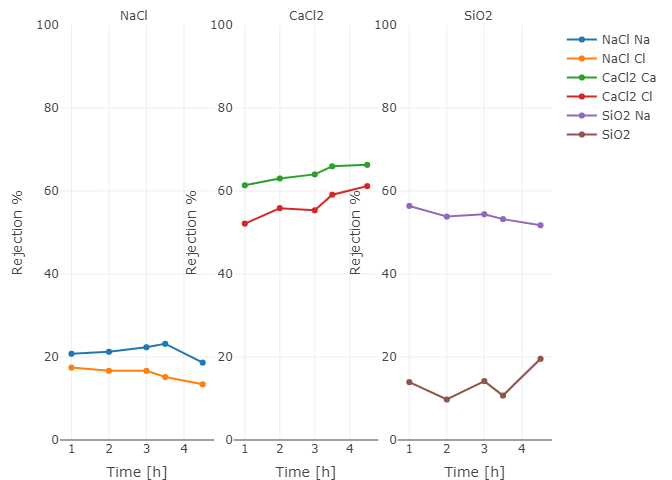
\includegraphics[width=0.9\textwidth]{Billeder/data/single_salt/Singlesalt_rejection_batch.png}
    \caption{Rejection of anions and cations from respective single salt filtrations \ce{NaCl}, \ce{CaCl2} and \ce{SiO2} plotted against water recovery}
    \label{fig:single_salt_rejection_summary}
\end{figure}


When comparing the \ce{Cl-} rejection from filtrations of \ce{NaCl} and \ce{CaCl2} it is evident that the \ce{Cl-} rejection is influenced by the corresponding cations present; when the monovalent \ce{Na+} is present the rejection of \ce{Cl-} decrease slightly from 17 \% to 13 \% during the filtration. 
Whereas when divalent \ce{Ca^{2+}} is present the \ce{Cl-} rejection is 52 \% increasing to 61 \%. 
This indicates a trend with increase in \ce{Cl-} rejection when divalent cations are present compared to monovalent cations.
This phenomenon is due to the larger divalent \ce{Ca^{2+}} ions have higher rejection %of 61 \% increasing to 66 \%, 
compared to monovalent \ce{Na+} ions. %with rejection of approx. 20 \%. 
This larger rejection can be due to larger stoke-Einstein radius of \ce{Ca^{2+}} = 0.309 nm compared to \ce{Na+}= 0.184 nm leading to larger steric size exclusion for \ce{Ca^{2+}}. 
%The negative membrane charge might also influence the two ions differently.

This trend of cations influence on \ce{Cl-} was also observed by single pass setup filtrations with same type of membrane, performed in previous internal work at Grundfos \citep{Sebastians_master_2020}. 
The rejection of 1.5 mM \ce{CaCl2} was found to be 68 \% and rejection of 1.5 mM \ce{NaCl} found to be 36 \%. \citep{Sebastians_master_2020}
Rejection of both these filtrations are significantly higher than those found in filtrations performed in relation to this project. 
This might be due to change in filtration parameters where the Internal Grundfos Study \citep{Sebastians_master_2020} had greater permeate flux of 30 LMH compared to 20 LMH for filtations made in the report, this could explain some of the performance differences.


For the \ce{Na2OSiO2} filtration there is a larger difference between rejection of cation \ce{Na+} and \ce{SiO2}, as \ce{Na+} has rejection of 56 \% decreasing to 52 \%. 
The \ce{SiO2} rejection was significantly lower and varies over time with 14 \% initially increasing to 20 \%. 
The initial silica rejection is comparable to previous internal work at Grundfos \citep{Sebastians_master_2020} where a silica rejection of 12 \% was achieved.
The \ce{SiO2}  charge should be considered, which is pH dependent, this filtration is performed with pH 8.5 where about 5 \% of \ce{SiO2} is assumed to be negatively charged, and the remaining neutral, according to \cref{fig:silica_pH_fraktion}.
This discrepancy between \ce{SiO2} rejection and \ce{Na+} rejection gives no charge neutrality if only these two ions are considered, this might indicate interference from other anions e.g. \ce{HCO3-}. 

% All three filtration found higher rejection of cations compared to the respective anions. 
% As there should exist charge neutrality over the membrane, \citep{wangPoreModelNanofiltration2021} the expected result is to find similar retention of anions and cations, especially in the simplified case of binary dissolved salt.
% %For the case of \ce{CaCl2} \citep{Sebastians_master_2020} found \ce{Cl-} and \ce{Ca^{2+}} rejections of 68\% and 69\%  respectively. 
% %Ignoring the difference in performance seen by our results, there is a large difference in charge balance: \ce{Cl-} rejection is 52 \% increasing to 61 \%, and \ce{Ca^{2+}} have higher rejection of 61 \% increasing to 66 \%. 
% This lack in charge neutrality could indicate other ions present influencing the charge balance such as bicarboante, or uncertainty of the analysis method used to determine the concentration. 



%\textbf{Bicarbonate discrepancy}

Along with measuring the concentrations of the ions which constitute the added binary salts the bicarbonate content of the feed stream was also analysed. 
%Progression of measured bicarbonate content is shown in \cref{fig:single_salt_bicarbonate} for each of the experiments.
For each experiment bicarbonate concentration increases in the feed container as the experiment progressed \ce{NaCl} and \ce{CaCl2} had initial bicarboante concentration of 0.14 and 0.10 mM respectively, which is significantly lower than the inital bicarboante concentration of \ce{Na2OSiO2} of 2.1 mM, see \rod{appendix single salt} for raw data. 
%There is a large difference in the initial bicarbonate concentration between the solutions of dissolved salts and the experiment on the silica solution.
%The analysis of bicarbonate is based on a titration to specific pH where bicarbonate content is assumed to be directly proportional to the volume of acid required to reach the target pH.
The analysis of bicarbonate is based on a titration and  silica can also contribute to the buffer capacity, as mentioned in \cref{Calcium_carbonate_carbonatesystem_teori}.  
This indicates that the analysis may be a result of the greater buffer capacity of the solution due to silica rather than an increased bicarbonate content.  


%\textbf{pH discrepancy}

%Before every experiment pH of the feed solution was adjusted to the desired pH of 8.5. %using 2M \ce{HCl} or 2M \ce{NaOH} .
During the filtration pH was logged and the measured pH varies between each filtration, even after initial adjustment to pH 8.5 results are shown in \rod{appendix single salt}. 
The initial pH had decreased to pH 7.3 for solution of \ce{NaCl} and to pH 8.1 for the \ce{CaCl2} binary solution.
Only the filtration containing silica achieved the initial pH of 8.5 and remained stable. 
This also indicates that the silica solution contributes to increased buffer capacity of solution. \citep{WaterChemistry1980} 
%For the two salt solutions \ce{NaCl} and \ce{CaCl_2} pH decreased as the filtration progressed while it remained constant for the silica solution, which is another indicator that the buffering capacities differ between the solutions.

\rod{Man kunne godt skrive noget her om alle de titreinger vi har lavet af CT vand, måske vi kan lave en Auto titreing af det CT vand vi får i uge 12}

%\textcolor{blue}{Skal der stå her at vi laver buffer frem over eller i Multi salt?}

% \begin{figure}[htbp]
%     \centering
%     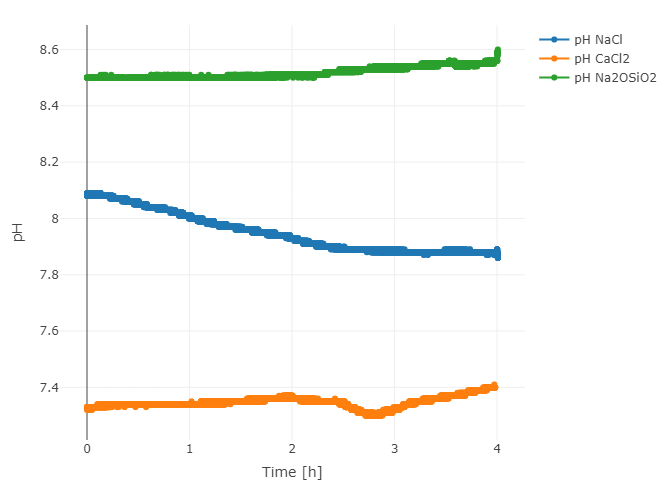
\includegraphics[width=0.7\textwidth]{Billeder/data/single_salt/Singlesalt_pH.png}
%     \caption{pH during filtration }
%     \label{fig:single_salt_pH}
% \end{figure}








